% Created 2016-06-08 Wed 09:22
\documentclass[presentation]{beamer}
\usepackage[utf8]{inputenc}
\usepackage[T1]{fontenc}
\usepackage{fixltx2e}
\usepackage{graphicx}
\usepackage{grffile}
\usepackage{longtable}
\usepackage{wrapfig}
\usepackage{rotating}
\usepackage[normalem]{ulem}
\usepackage{amsmath}
\usepackage{textcomp}
\usepackage{amssymb}
\usepackage{capt-of}
\usepackage{hyperref}
\usetheme{Frankfurt}
\usecolortheme{}
\usefonttheme{}
\useinnertheme{}
\useoutertheme{}
\author{Daniel Kessler}
\date{\textit{<2016-06-08 Wed>}}
\title{Growth Charting of Brain Connectivity Networks and the Identification of Attention Impairment in Youth}
\subtitle{Published in JAMA Psychiatry, 2016 (Kessler, Sripada, \& Angstadt)}

\hypersetup{
 pdfauthor={Daniel Kessler},
 pdftitle={Growth Charting of Brain Connectivity Networks and the Identification of Attention Impairment in Youth},
 pdfkeywords={},
 pdfsubject={},
 pdfcreator={Emacs 24.3.1 (Org mode 8.3.4)}, 
 pdflang={English}}
\begin{document}

\maketitle
\begin{frame}{Outline}
\tableofcontents
\end{frame}




\section{Introduction}
\label{sec:orgheadline3}
\stepcounter{subsection}
\begin{frame}[label={sec:orgheadline1}]{Motivation}
\begin{block}{Pediatric Growth Charts}
\begin{itemize}
\item Long history for height, weight, etc
\end{itemize}
\end{block}
\begin{block}{Intrinsic Connectivity Networks}
\begin{itemize}
\item Attention \& ADHD connection
\item DMN vs TPN balance
\end{itemize}
\end{block}
\end{frame}
\begin{frame}[label={sec:orgheadline2}]{Background}
\begin{itemize}
\item Focus today: processing pipeline, modeling, and analysis
\item Slides: linked from \url{http:dankessler.me}
\item Paper: \href{http://archpsyc.jamanetwork.com/article.aspx?articleid=2513687}{Kessler, Angstadt, \& Sripada. JAMA Psychiatry 2016}
\end{itemize}
\end{frame}
\section{Methods}
\label{sec:orgheadline19}
\stepcounter{subsection}
\begin{frame}[label={sec:orgheadline4}]{Method Overview}
\begin{figure}[htb]
\centering
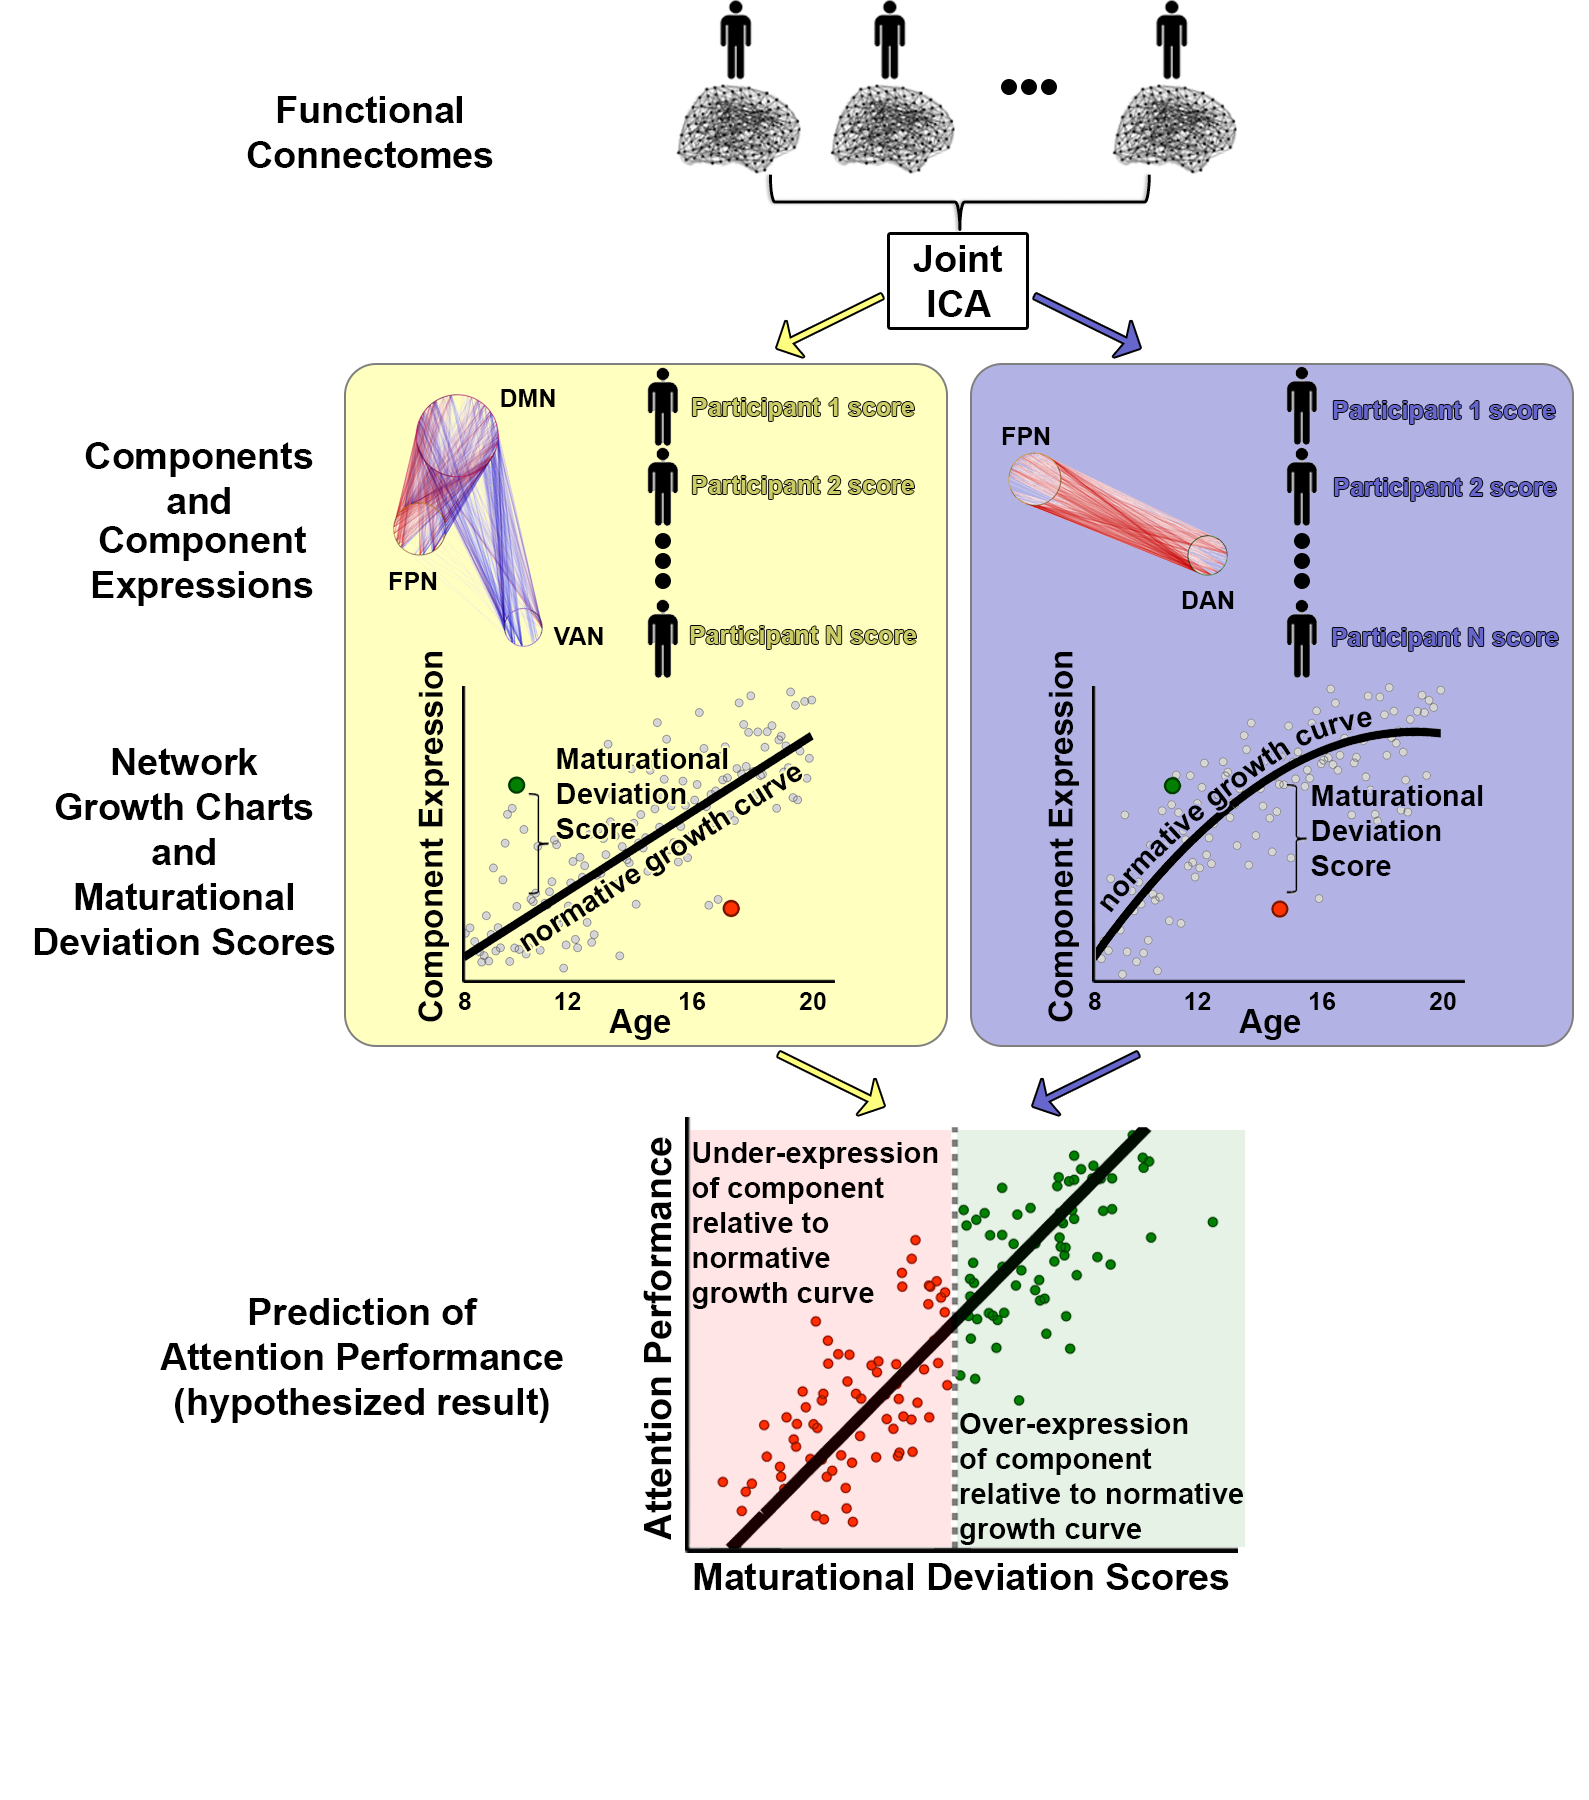
\includegraphics[height=7.75cm]{./Figures/Figure1.png}
\end{figure}
\end{frame}
\begin{frame}[label={sec:orgheadline5}]{Sample}
\begin{figure}[htb]
\centering
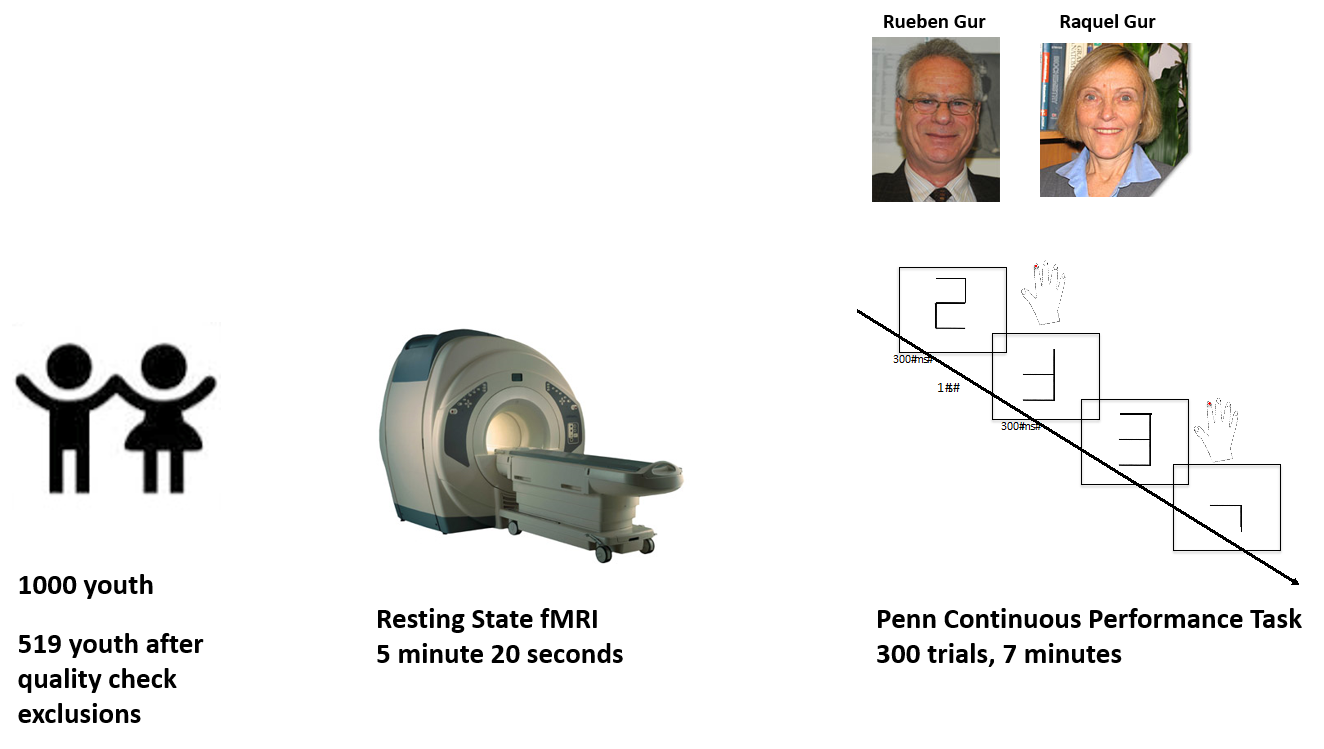
\includegraphics[height=4cm]{./Figures/PNC.png}
\end{figure}
\begin{itemize}
\item Philadelphia Neurodevelopmental Cohort
\item Resting state fMRI
\item Penn Continuous Performance Task
\item N = 519 (after QC \& exclusions)
\end{itemize}
\end{frame}

\begin{frame}[label={sec:orgheadline6}]{Task: PCPT}
\begin{itemize}
\item Penn Continuous Performance Test
\item 180 trials
\item 1s to respond
\item "Go" on digit/letter (varies by phase)
\item Measure: Acc (corrected for age with quadratic model)
\end{itemize}
\end{frame}
\begin{frame}[label={sec:orgheadline7}]{Clinical Interview}
\begin{itemize}
\item Assesses psychopathology dimensions
\item ADHD Module
\item Symptom endorsement -> pseudo ADHD "diagnosis"
\end{itemize}
\end{frame}
\begin{frame}[label={sec:orgheadline8}]{MRI Measures}
\begin{itemize}
\item T1-weighted image (structural contrast)
\item Resting State fMRI
\end{itemize}
\begin{block}{T1 Image}
\begin{itemize}
\item Structural contrast
\item Ventricles are black, "gray matter" is darker, "white matter" is brither
\end{itemize}
\end{block}
\begin{block}{Resting state fMRI}
\begin{itemize}
\item 4D Image (Multiple "Volumes"): X*Y*Z*time
\item T2* contrast captures BOLD (blood oxygenation, coupled to neural activity)
\end{itemize}
\end{block}
\end{frame}
\begin{frame}[label={sec:orgheadline9}]{fMRI Prepocessing Overview}
Lots of quality-control steps throughout
\begin{enumerate}
\item Slice-time Correction
\item Motion Correction
\item Normalization
\item Smoothing
\end{enumerate}
\end{frame}
\begin{frame}[label={sec:orgheadline10}]{Preproc: Slice-time Correction}
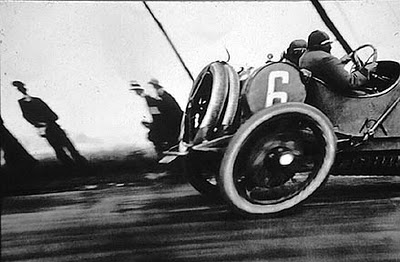
\includegraphics[width=3cm]{./Figures/rollingshuttercar.jpg}
\begin{itemize}
\item Each fMRI volume is acquired sequentially in slices
\item Volume not acquired simultaneously
\item Correct (through interpolation) s.t. all slices w/in volume temporally aligned
\end{itemize}
\end{frame}
\begin{frame}[label={sec:orgheadline11}]{Prepoc: Motion Correction}
\begin{itemize}
\item Participants move their head over the scan
\item Estimate affine realignment to common volume (e.g. V\(_{\text{0}}\))
\item Alignment is progressive (rigid body transforms)
\begin{itemize}
\item realign V\(_{\text{1}}\) to V\(_{\text{0}}\) using affine matrix Q\(_{\text{1}}\)
\item align V\(_{\text{2}}\) to V\(_{\text{0}}\), initialize solution with Q\(_{\text{1}}\)
\item and so on
\end{itemize}
\item Store Q\(_{\text{i}}\)
\item Process Q\(_{\text{i}}\)'s to capture summary displacement information for each frame
\begin{itemize}
\item this will be used later in preproccessing
\end{itemize}
\end{itemize}
\end{frame}
\begin{frame}[label={sec:orgheadline12}]{Preproc: Normalization}
\begin{itemize}
\item Everybody's brain is unique
\item This is problematic for group analyses
\item Standard Brain/Space: MNI (Montreal Neurological Institute)
\item Steps
\begin{enumerate}
\item Rigid body registration of T1 scan to T2* scan
\item Estimate nonlinear warp (affine + splines) b/w T1 and MNI template
\item Apply estimated warp to each volume of T2* scan
\end{enumerate}
\end{itemize}
\end{frame}
\begin{frame}[label={sec:orgheadline13}]{Preproc: Smoothing}
\begin{itemize}
\item Normalization isn't perfect
\item Brains are plastic and diverse even when perfectly aligned anyway
\item Smooth with Gaussian kernel (3D, 8mm FWHM)
\end{itemize}
\end{frame}
\begin{frame}[label={sec:orgheadline14}]{Resting Processing \& Connectome Generation}
\begin{block}{Processing}
\begin{itemize}
\item Linearly detrended
\item COMPCor: PCA-based nuisance regression (CSF \& WM)
\item Bandpass Filtering (0.01 to 0.1 Hz)
\item Motion Scrubbing: Delete volumes with large displacement/motion
\end{itemize}
\end{block}
\begin{block}{Connectome Generation}
\begin{itemize}
\item Isomorphic grid, 12mm spacing
\item 1068 Regions of Interest (ROIs)
\item Calculate pairwise correlation, then R-to-Z transform
\item Vector embedding: Each participant contributes \({1068}\choose{2}\) edges
\end{itemize}
\end{block}
\end{frame}
\begin{frame}[label={sec:orgheadline15}]{Data Cleansing}
\begin{itemize}
\item Intersubject nuisance effects may manifest at edge level
\item e.g.: left handers have > connectivity at edge i
\item Concatenate vector embeddings into matrix X
\item estimate with OLS \(X = Y\hat{\beta} + \hat{\epsilon}\)
\item Reestimate data as \(X^{\dagger} = Y^{\dagger}\hat{\beta}\)
\item Y\(^{\textdagger{}}\) is ideal design matrix where nuisance fx are flat
\item Induce eigenvector selection through augmentation: add \(\hat{\beta}\) for fx of interest at each edge
\end{itemize}
\end{frame}
\begin{frame}[label={sec:orgheadline16}]{Independent Components Analysis}
\begin{itemize}
\item reduce rows of \(X^{\dagger}\) through PCA (\(DX\)) (retain top 15 eigenvectors)
\item ICA-decomposition using FastICA \(X=AS\)
\item A: mixing matrix 15 by 15
\item S: source matrix: 15 by \({1068}\choose{2}\)
\item Unreduce \(A^{\dagger}=D^{-1}A\)
\item \(A^{\dagger}\) is \# of subjects by 15
\item The i,j element indicates the expression of component j for subject i
\end{itemize}
\end{frame}
\begin{frame}[label={sec:orgheadline17}]{Network Assignment \& Visualization}
\begin{figure}[htb]
\centering
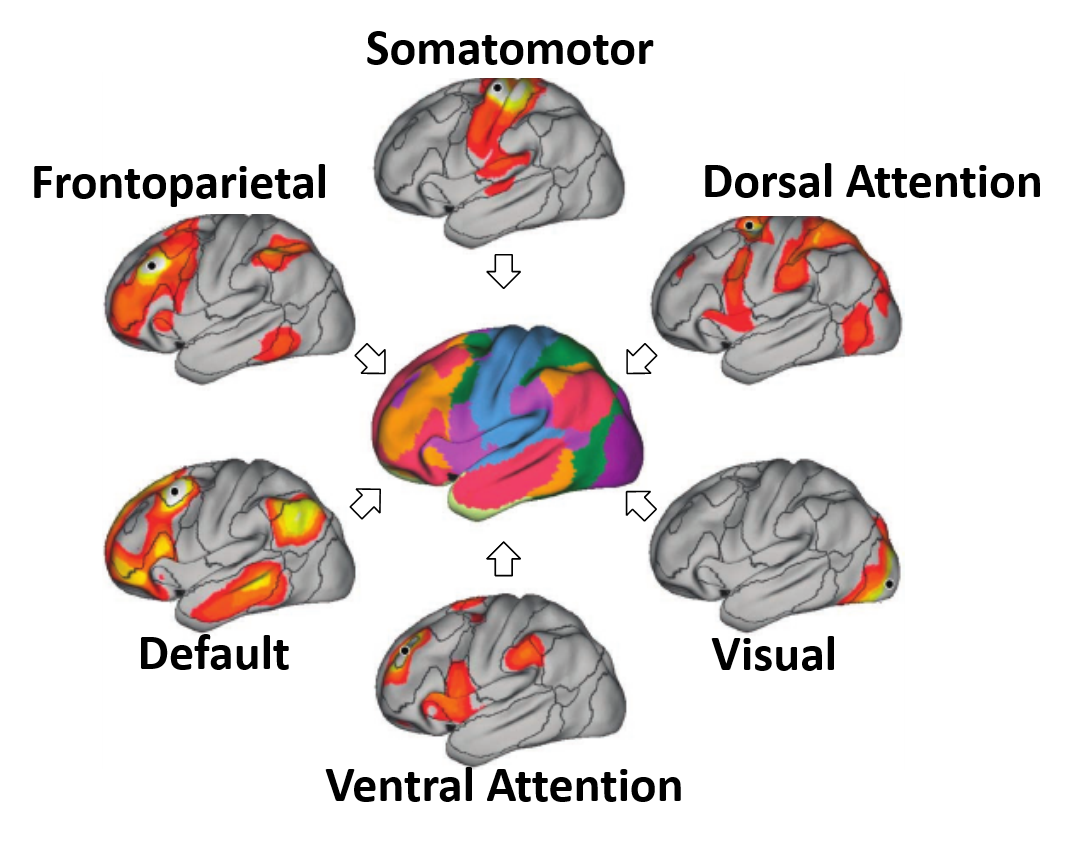
\includegraphics[height=6cm]{./Figures/Yeo1.png}
\end{figure}
\begin{figure}[htb]
\centering
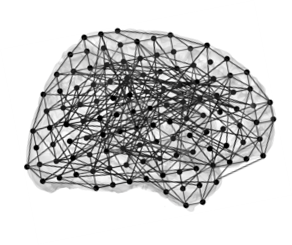
\includegraphics[height=1.5cm]{./Figures/Yeo2.png}
\end{figure}

Buckner et al. Opportunities and limitations of intrinsic functional connectivity MRI. Nature Publishing Group (2013) vol. 16 (7) pp. 832-837
\end{frame}

\begin{frame}[label={sec:orgheadline18}]{Network Growth Charting Analyses}
\begin{itemize}
\item Growth charts obtained from OLS population-level estimates
\item Predict each column of A with OLS \(A^{\dagger}_i = age + age^2\)
\item Residuals from these models are \alert{deviation scores} reflecting over- or under- expression of a component relative to age
\item Use \alert{deviation scores} to predict
\begin{itemize}
\item Accuracy on PCPT (age-corrected)
\item ADHD status
\end{itemize}
\end{itemize}
\end{frame}
\section{Results}
\label{sec:orgheadline25}
\stepcounter{subsection}
\begin{frame}[label={sec:orgheadline20}]{Network Growth Charting to Predict Task Accuracy}
\begin{itemize}
\item \alert{Deviation scores} predict accuracy very well (R\(^{\text{2}}\) = 0.287)
\item A subset of just 6 components' \alert{deviation scores} do most of the work (R\(^{\text{2}}\) = 0.240)
\item Of these, 5 show vigorous maturational profiles
\item Split half analysis, OLS with all 15 \alert{deviation scores}: R\(^{\text{2}}\) = 0.176
\end{itemize}
\begin{figure}[htb]
\centering
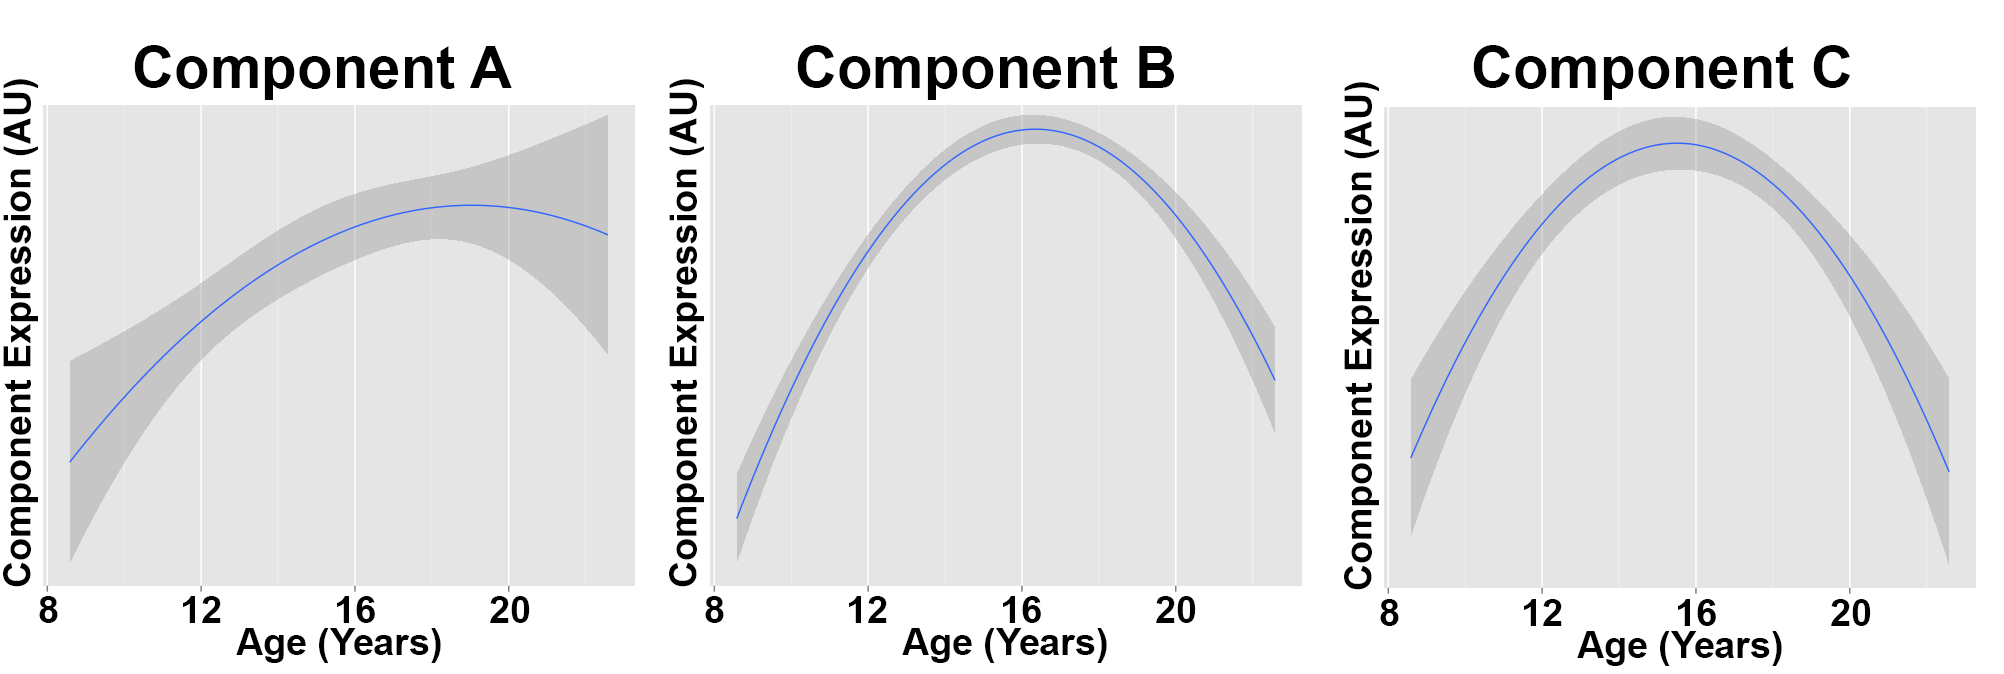
\includegraphics[height=3cm]{./Figures/Figure3.png}
\end{figure}
\end{frame}
\begin{frame}[label={sec:orgheadline21}]{DMN-TPN Shifts in Maturing Components}
\begin{figure}[htb]
\centering
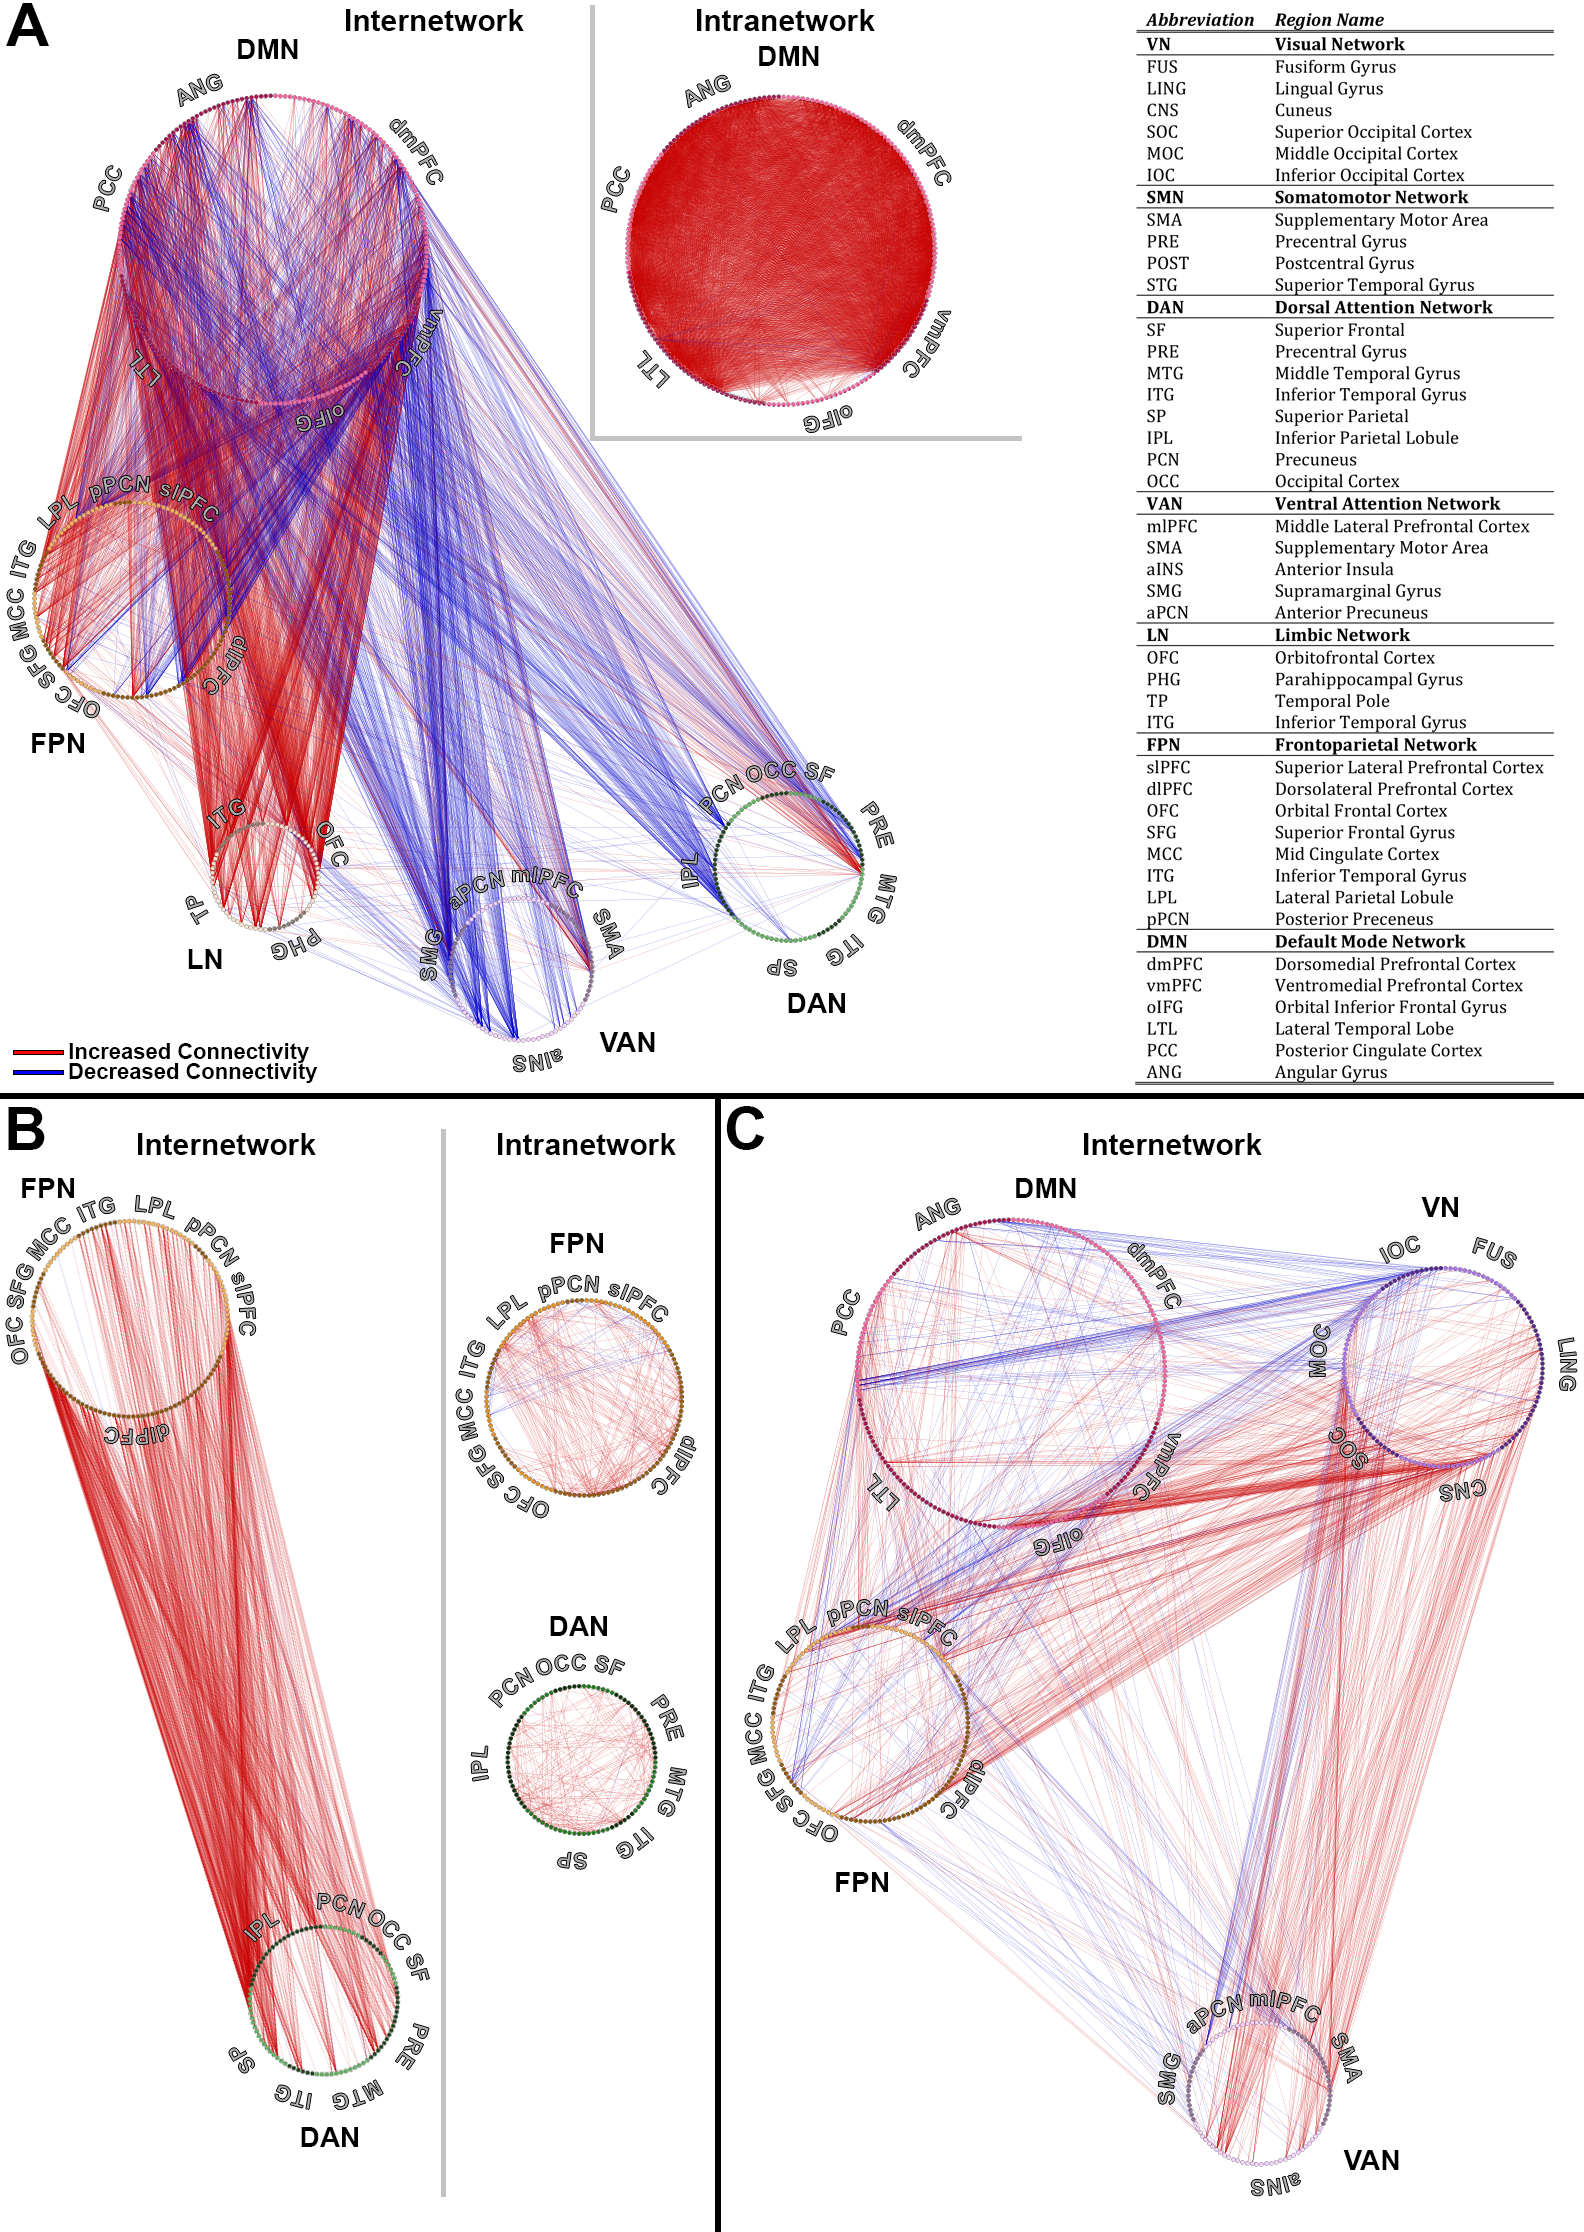
\includegraphics[height=7.75cm]{./Figures/Figure2.png}
\end{figure}
\end{frame}
\begin{frame}[label={sec:orgheadline22}]{Shallow vs Lagged Dysmaturation and Task Accuracy}
\begin{figure}[htb]
\centering
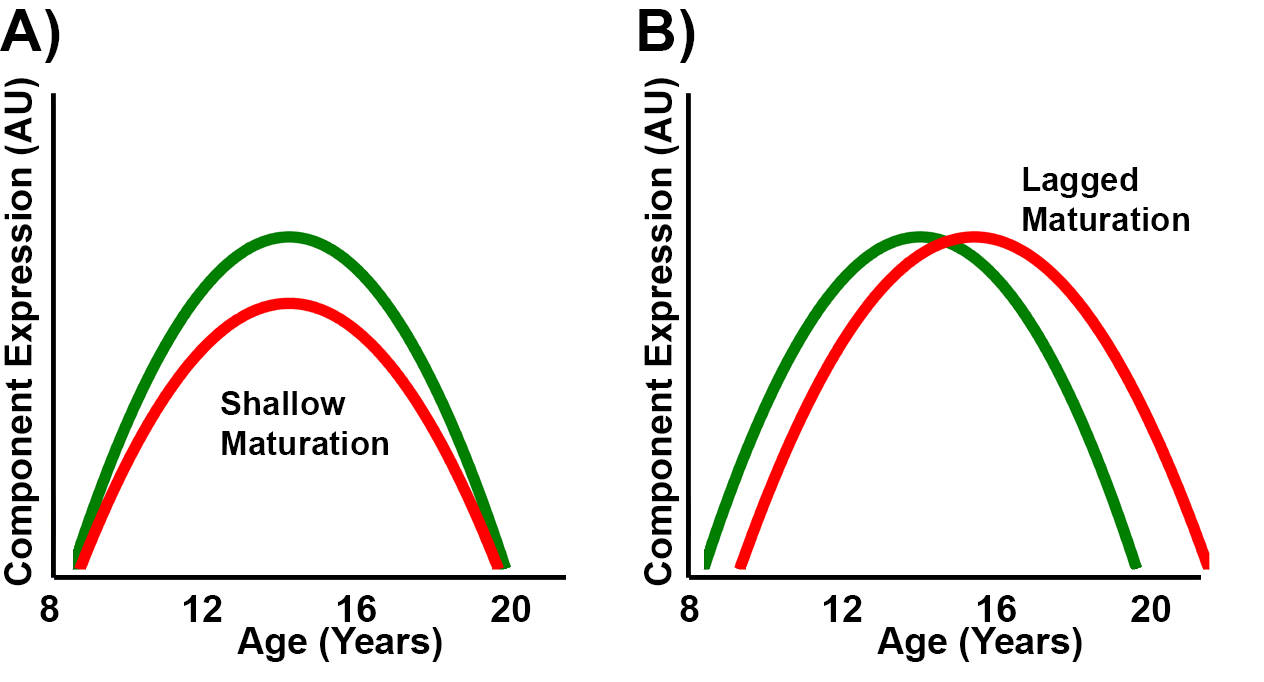
\includegraphics[height=4cm]{./Figures/eFig7.png}
\end{figure}
\begin{columns}
\begin{column}{.5\columnwidth}
\alert{Shallow Dysmaturation}
Dysmaturation yields consistent underexpression of components
\end{column}
\begin{column}{.5\columnwidth}
\alert{Lagged Dysmaturation}
Dysmaturation yields comparable, but right-shifted, peak
\end{column}
\end{columns}
\begin{block}{Strong Evidence for Shallow Dysmaturation over Lagged}
Likelihood Ratio > 10\(^{\text{26}}\)
\end{block}
\end{frame}
\begin{frame}[label={sec:orgheadline23}]{Biomarker of Attention Dysfunction from Network Growth Charting}
\begin{itemize}
\item Goal: Binary Classification of Attention Dysfunction
\item Binarize task performance into \emph{low} and \emph{normal} performers (split by \%ile cutoff)
\item Vary \%ile cutoff for binning
\item LOOCV of Logistic Regression, performance assessed with ROC AUC, error bars from permutations
\end{itemize}
\begin{figure}[htb]
\centering
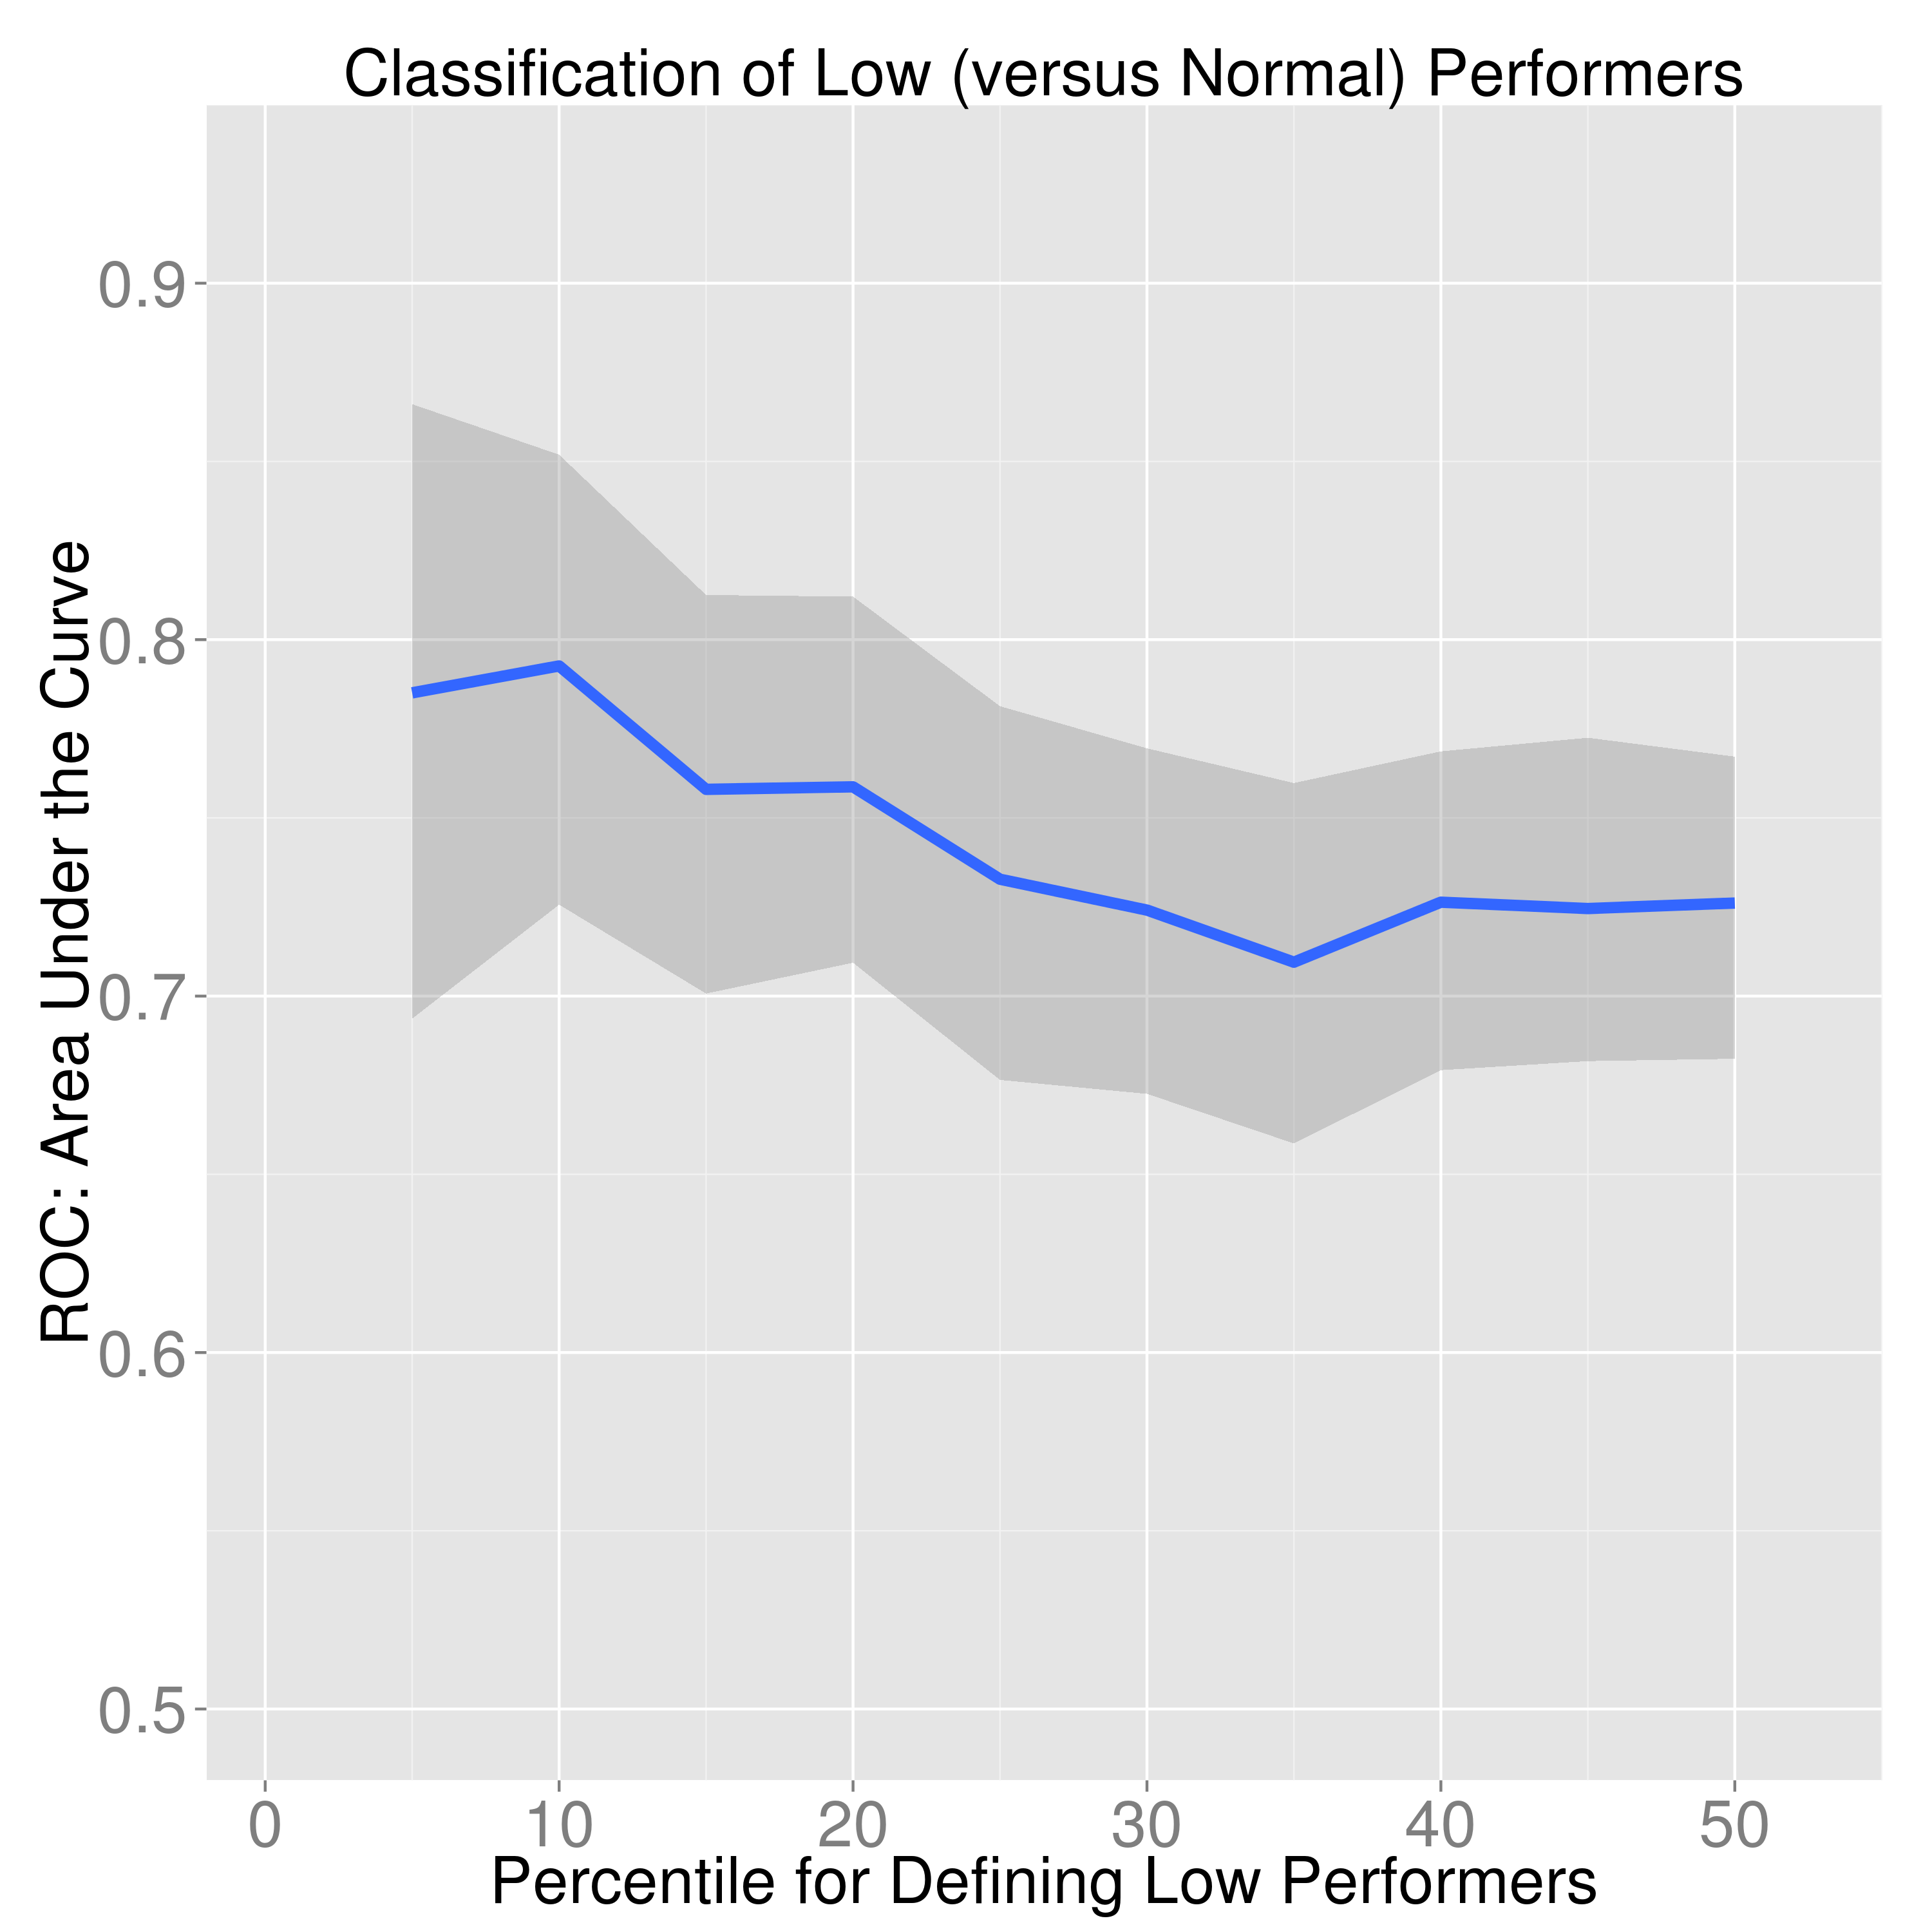
\includegraphics[height=3cm]{./Figures/Figure4.png}
\end{figure}
\end{frame}
\begin{frame}[label={sec:orgheadline24}]{Biomarker of ADHD from Network Growth Charting}
\begin{itemize}
\item Goal: Binary Classification of Pseudo ADHD Diagnosis
\item Logistic regression predicting dx using 6 components IDed earlier
\item Model is significant, but effect size weak compared to attention prediction
\item \(\chi^2_6 = 13.00; P = 0.043\)
\end{itemize}
\end{frame}
\section{Discussion}
\label{sec:orgheadline27}
\stepcounter{subsection}
\begin{frame}[label={sec:orgheadline26}]{Discussion}
\begin{itemize}
\item Recent review paper calls for developmental approaches to connectomic imaging
\item We link dysmaturation of ICN topology to attention dysfunction
\item DMN-TPN intra- and inter-relationships implicated
\item Shallow vs lagged dysmaturation provides better predictive fit
\end{itemize}
\end{frame}
\section{Acknowledgements}
\label{sec:orgheadline28}
\begin{itemize}
\item Chandra Sripada (PI)
\item Mike Angstadt (Research Computer Specialist)
\item Yu Fang (Processing)
\end{itemize}
\end{document}
